The interaction of light with any other object is described best with a set of 
equations called the Maxwell equations. This set of equations fully capture and 
describes the electromagnetic wave nature of light. It relates point wise the 
electric wave vector $\vb{E}$, the magnetic induction $\vb{B}$, the electric 
current density $\vb{j}$, the electric displacement $\vb{D}$, and the magnetic 
vector $\vb{H}$ with each other for objects where the physical properties are 
continuous in the neighbourhood of the point of interest~\cite{Born1980Ch1}
\begin{subequations}
  \begin{align}
    \curl{\vb{H}} - \frac{1}{c}\pdv{t}\vb{D} &=\frac{4\pi}{c}\vb{j} 
    \label{eq:Th-ampere} \\
    \curl{\vb{E}} - \frac{1}{c}\pdv{t}\vb{B} &=  0
    \label{eq:Th-faraday} \\
    \div{\vb{D}} &= 4\pi\rho_{\MR{E}}
    \label{eq:Th-gauss} \\
    \div{\vb{B}} &= 0
    \label{eq:Th-gauss-mag}
  \end{align}
\end{subequations}
with $c$ being the speed of light and $\rho_{\MR{E}}$ the total electric charge 
density. Although, 
\cref{eq:Th-ampere,eq:Th-faraday,eq:Th-gauss,eq:Th-gauss-mag} describe the 
behavior of light fully, it is often more convenient to think of light as a 
collection of single rays. In the limit of a vanishing small light wavelengths 
$\lambda_{\text{light}}$ compared to the object size $R$, the approximation of 
light as single rays is valid~\cite{Born1980Ch3}. This branch of describing the 
propagation of light is called -- amongst others -- \emph{Ray Optics}.

Our laser has a wavelength of $\lal=\SI{785}{\nm}$ and the smallest object we 
use has a radius of $R=\SI{1.03}{\um}$. The ratio $\sfrac{2R}{\lal}\approx 2.6$ 
is close to unity and the application of ray optics in our case might be 
questionable. However, previous works with our optical trap
\cite{Lakaemper2015,Lamprecht2016,Lamprecht2017} have shown that the ray 
approximation is a reasonable approach in our case. In addition, one has to 
differentiate between quantitative and qualitative analysis. In all here 
presented results we use our optical trapping setup as tool for relating 
results qualitatively.

\section{Experimental Setup}

\begin{figure}[htp]
  \centering
  % \tikzsetnextfilename{setup}

  \definecolor{tempcolor}{RGB}{176, 206, 255}
\pgfmathdeclarefunction{gauss}{2}{%
  \pgfmathparse{1/(#2*sqrt(2*pi))*exp(-((x-#1)^2)/(2*#2^2))}%
}

\begin{tikzpicture}

  \shade[top color=white,bottom color=white,middle color=red] (3,-0.15) 
  rectangle ++(2.5,0.3);

  \shade[top color=white,bottom color=white,middle color=red] (5.5,-1.25) 
  rectangle (10,1.25);

  % laser head
  \filldraw[color=black,fill=black!50] (0,-0.5) rectangle ++(3,1);
  \node at (1.5,0) {Laser head};

  % lens
  \fill[tempcolor] (5.5,0) ellipse (0.15 and 1.5);
  \path (5,1.5) -- ++(1,0) node[above, midway, anchor=south] {Expanding lens};

  % microscope
  \filldraw[white] (9,-2) rectangle ++ (2,4);
  \filldraw[black] (9,-0.2) rectangle (9.2,-1.5);
  \filldraw[black] (9,0.2) rectangle (9.2,1.5);
  \filldraw[red] (9,-0.2) rectangle ++(1.5,0.4);

  \draw[black,thick] (10,-1) -- ++(0,0.8) -- ++(0.3,0) -- ++(0,0.4) -- 
  ++(-0.3,0) -- ++(0,0.8);

  \path (7.0,1.5) -- ++(4,0) node[above, midway, anchor=south, align=center] 
  {Microscope housing};

  \draw[black, very thick, ->] (11,0) -- ++(1.5, 0) -- ++(0, -4) -- ++(-1.5,0);

  \draw[black!70, thin] (7,-0.21) -- ++(2,0);
  \draw[black!70, thin] (7,+0.21) -- ++(2,0);

  %% bottom
  \fill[tempcolor] (10,-4) ellipse (0.15 and 0.75);
  \path (9.5,-3.25) -- ++(1,0) node[above, midway, anchor=south] {Focussing 
  lens};

  \coordinate (M) at (8.5,-4);
  \draw[black,thin,->] (M) -- node[above,pos=0.9] {\tiny$\ex$} ++(0,0.5);
  \draw[black,thin,->] (M) -- node[above,pos=0.9] {\tiny$\ey$} ++(0.4,0.4);
  \draw[black,thin,->] (M) -- node[above,pos=0.9] {\tiny$\ez$} ++(-0.5,0);
  \shade[ball color=black!10] (M) circle (.25);

  \path (8.25,-4.5) -- ++(0.5,0) node[below, midway] {particle};

  \fill[tempcolor] (7.0,-4) ellipse (0.15 and 0.75);
  \path (6.5,-3.25) -- ++(1,0) node[above, midway, anchor=south] {Condensor 
  lens};

  \filldraw[color=black, fill=black!50] (5.5,-4.5) rectangle ++(-1,1);
  \path (4.5,-4.5) -- ++(1,0) node[below, midway, anchor=north] {Filter};

  \fill[tempcolor] (2.5,-4) ellipse (0.15 and 0.75);
  \path (2,-3.25) -- ++(1,0) node[above, midway, anchor=south] {Lens 3};

  \filldraw[color=black, fill=black!10] (0,-4.4) rectangle ++(0.8,0.8);
  \draw[thick,black,dotted] (0,-4) -- ++(0.8,0);
  \draw[thick,black,dotted] (0.4,-4.4) -- ++(0,0.8);

  \path (0,-3.5) -- ++(0.8,0) node[above, midway, anchor=south] {QPDs};
  \filldraw[color=red!50] (0.4,-4) circle (.2);

  \draw[red, thick] (11, -3.6) -- ++(-1,0) -- ++(-3,-0.8) -- (5.5,-4.4);
  \draw[red, thick] (11, -4.4) -- ++(-1,0) -- ++(-3,+0.8) -- (5.5,-3.6);
  \draw[red!50, thick, dashed]  (4.5,-4.4) -- (2.5,-4.4) -- (0.4,-3.8);
  \draw[red!50, thick, dashed]  (4.5,-3.6) -- (2.5,-3.6) -- (0.4,-4.2);


\begin{axis}[
    domain=-0.15:0.15,
    samples=200,
    no markers,
    axis lines=none,
    ticks=none,
    xmin=-1,
    xmax=1,
    ymax=250,
    anchor = origin,
    rotate around={270:(current axis.origin)},
    hide axis,
    yshift=36mm
    ]

    \addplot[black] {gauss(0,0.01)};

\end{axis}

\begin{axis}[
    domain=-0.3:0.3,
    samples=100,
    no markers,
    axis lines=none,
    ticks=none,
    xmin=-1,
    xmax=1,
    ymax=20,
    anchor = origin,
    rotate around={270:(current axis.origin)},
    hide axis,
    yshift=65mm
    ]

    \addplot[black] {gauss(0,0.15)};

\end{axis}

\end{tikzpicture}

  \includegraphics[]{Plots/cache/setup.pdf}
  \caption{Schematic of light path from laser head to quadrant photo detectors. 
  In the top half sketch red shading and the black lines the laser intensity 
profile qualitatively. In the bottom half just the outer most laser rays are 
depicted.}
  \label{fig:Th-setup}
\end{figure}

Before highlighting important parts from ray optics it is advantageous to 
understand our optical trapping setup which is based upon the work of Arthur 
Ashkin~\cite{Ashkin1978,Ashkin1987,Ashkin2002,Ashkin1986,Ashkin1992,Ashkin1997}. 
\cref{fig:Th-setup} depicts a basic schematic of the laser path from the laser 
source to the quadrant photo detectors (QPDs) in the back focal plane. A 
complete overview of our setup with a list and explanation of every used part 
is available in~\cite{Lamprecht2017}.

Our laser diode emits a tightly confined laser beam in the near-infrared regime 
(non-visible) with a wavelength of $\lal=\SI{785}{\nm}$ and a maximal power of 
$P=\SI{200}{\milli\watt}$ and with a transverse electromagnetic mode of order 
00 (TEM$_{00}$). This laser profile is axisymmetric to the light propagation 
direction and can be visualized with a rotating Gaussian bell curve. Next, the 
beam is expanded such that it is much larger than the opening of the microscope 
housing. The magnitude of the trapping forces are proportional to the laser 
intensity of the beam. The biggest contribution to the total force stems from 
the outer parts of the beam. Therefore, it is advantageous to broaden the beam 
before guiding it to the focusing lens. The opening of the microscope is 
overfilled by the broadened beam and the laser intensity after this cutoff can 
be approximated with a flat-top profile. Hence, every light wave (also the ones 
contributing most to the total trapping force) carries the same intensity.

The next step is the focusing of the beam with a high numerical aperture (NA) 
oil immersion lens. Here, the actual trapping of the particle occurs. If more 
than just the trapping of particles is of interest, the beam needs to be 
investigated further. The relative movement of the particle within the trap 
contains the necessary information. In order to image the movement in the $\ex$ 
and $\ey$ direction the beam is collimated again by the condensor lens after it 
passed the particle and filtered to reduce its total intensity to prevent 
damage of the QPDs. Before the beam is focussed, it is split into two because 
the axial movement detection for $\ez$ and the in plane movement detection for 
$\ex$ and $\ey$ have inherently different working principles.

If the particle moves within the trap the spot on the QPDxy will also move. By 
measuring the voltage on each quadrant of the QPDxy and summing and subtracting 
certain quadrants it is possible to retrieve the information about the movement 
in each direction separately. For the axial direction the opening of the QPDz 
is overfilled. An axial movement of the particle causes a change of total 
intensity on this QPD. By measuring the QPDz total intensity we have the 
information about the relative movement of the particle within the trap. After 
the calibration of the OT the measured voltages that are proportional to the 
particle movement can be converted to the physical unit meter. The calibration 
process itself is not relevant for this thesis but is available 
here~\cite{Lamprecht2017}. An discussion of different calibration options is 
available from \citeauthor{Svoboda1994}~\cite{Svoboda1994} and 
\citeauthor{Jun2004}~\cite{Jun2004}.

\section{Ray Optics\label{sec:Th-rayoptics}}

As said before, in the regime of ray optics the propagation of light is 
visualized by single rays. The interaction of a single ray at an interface is 
then studied geometrically. The defining property for these kind of 
investigations is the so called refractive index $\refraction$. Light travels 
in vacuum at speed of light $c=\SI{299792458}{\m\per\s}$. In other mediums than 
vacuum the speed of light has a different (smaller) magnitude. The refractive 
index relates the speed of light of vacuum $c$ to any other material $c_{\Box}$
\begin{equation}
  c_{\Box} = \frac{c}{n}.
  \label{eq:Th-lightspeed}
\end{equation}
Since there is nothing faster than the speed of light, the refractive index 
$\refraction$ cannot be smaller than 1. This index is not constant for one 
material but a function of the wavelength $\lambda$. Additionally, the 
refractive is in general a complex quantity
\begin{equation}
  \refraction\geq 1 \quad \wedge \quad \refraction \coloneqq 
  \refraction(\lambda) = \refraction(\lambda) - \iu\alpha(\lambda)
  \label{eq:Th-refractive-index}
\end{equation}
where $\alpha$ is called the absorption coefficient~\cite{Jackson2013}. Any ray 
of any wavelength is attenuated when propagating through any medium, e.g. in a 
depth of approximately \SI{1}{\kilo\meter} it is completely dark in the ocean 
because all the intensity of the sunlight is attenuated there. The absorption 
coefficient captures how fast this attenuation occurs.

\begin{figure}[htp]
  \centering
  % \tikzsetnextfilename{Snell}

\tikzstyle arrowstyle=[scale=1]

\tikzstyle directed=[postaction={decorate,decoration={markings,
    mark=at position .65 with {\arrow[arrowstyle]{stealth}}}}]

\tikzstyle reverse directed=[postaction={decorate,decoration={markings,
    mark=at position .65 with {\arrowreversed[arrowstyle]{stealth};}}}]

\tikzset{SnellNode/.style={text width=10mm, align=center}}

\begin{tikzpicture}
  \def\W{5}
  \def\H{4}
  \def\x{0.95}
  \def\anglealpha{0}
  \pgfmathsetmacro{\y}{{(1-\x)*\H}}
  \pgfmathsetmacro{\radius}{(\W^2+\y^2)/2/\y}
  \pgfmathsetmacro{\anglealpha}{{asin(\W/\radius)}}
  \pgfmathsetmacro{\s}{{90+\anglealpha}}
  \pgfmathsetmacro{\e}{{90-\anglealpha}}

  \pgfmathsetmacro{\anglebeta}{{0.8*\anglealpha}}
  \pgfmathsetmacro{\p}{{(\radius-\H)*sin(\anglebeta)}}
  \pgfmathsetmacro{\px}{{\radius*sin(\anglebeta)}}
  \pgfmathsetmacro{\py}{{-\radius*(1-cos(\anglebeta))}}


  % define coordinates
  \coordinate (O) at (0,0) ;
  \coordinate (A) at (0,\H) ;
  \coordinate (B) at (0,-\H) ;

  % media
  \fill[blue!20,opacity=.3] (-\W,0) rectangle (\W,\H);
  \fill[black!10!,opacity=.3] (-\W,0) rectangle (\W,-\H);
  \node[right, SnellNode] at (3,1.5) {{Fluid\\ $\nf$}};
  \node[left, SnellNode] at (-2,-2) {{Particle\\ $\ns$}};

  % axis
  \draw[dash pattern=on5pt off3pt] (A) -- (B) ;
  % normal
  \draw[|->, thick] (0,0) -- node[right, pos=1] {$\normalvector$} (0, 2.5);


  % ray representation
  \def\gamma{130}
  \draw[red, variable=\x, domain=2.5:\W, samples=100] (0,\H) plot 
  ({\x*cos(\gamma)-cos(\x*pi r*3)/4*sin(\gamma)},{sin(\gamma)*\x+cos(\x*pi 
  r*3)/4*cos(\gamma)});

  % rays
  \draw[red,ultra thick,reverse directed] (O) -- node[left, xshift=-1mm, 
  pos=0.2] {$P_{\MR{i}}$} (130:5.2);

  \draw[red,ultra thick,directed] (O) -- node[right, xshift=1mm, pos=0.2] 
  {$P_{\MR{r}}$} (50:5.2);

  \draw[red,thick,dotted] ([xshift=1cm]O) -- ([xshift=1cm]130:5.2);
  \draw[red,thick,dotted] ([xshift=1cm]O) -- ([xshift=1cm]50:5.2);

  \draw[red,|<->|,>=stealth'] (130:3) -- node[above,pos=0.2,yshift=1mm] 
  {$w_{\MR{i}}$} ++(+40:0.775);
  \draw[red,|<->|,>=stealth'] (50:4) -- node[above,pos=0.7] {$w_{\MR{r}}$} 
  ++(-40:0.775);

  \draw[blue,directed,ultra thick] (O) -- node[right, xshift=1mm, pos=0.2] 
  {$P_{\MR{t}}$} (-70:4.24);

  \draw[blue,thick,dotted] ([xshift=1cm]O) -- ([xshift=1cm]-70:4.24);

  \draw[blue,|<->|,>=stealth'] (-70:3) -- node[above,pos=0.4] {$w_{\MR{t}}$} 
  ++(20:0.945);

\draw[thick,|<->|,>=stealth'] (O) -- node[midway,below] {$w$} ++(1,0);

  % particle circumference
  \draw (-\W,-\y) arc (\s:\e:\radius);
  \draw[black,->|,>=stealth'] (\p,-\H) -- node[right, pos=0.7] {$\R$} (\px, 
  \py);

  % angles
  \draw[->,>=stealth'] (0,1) arc (90:130:1);
  \draw[->,>=stealth'] (0,1) arc (90:50:1);
  \draw[->,>=stealth'] (0,-1.4) arc (270:290:1.4);

  \node[] at (280:1.8)  {$\transmitted$};
  \node[] at (110:1.4)  {$\incident$};
  \node[] at (70:1.4)  {$\reflected$};

\end{tikzpicture}

  \includegraphics[]{Plots/cache/Snell.pdf}
  \caption{Visualization of \emph{Snell's Law} for rays at an interface of two 
  media with different refractive indices $\refraction_{\Box}$.}
  \label{fig:Th-Snell}
\end{figure}

The most important relation in the ray optics regime is \emph{Snell's Law} (see 
also \cref{fig:Th-Snell})
\begin{equation}
  \nf\,\sin\incident = \ns\,\sin\transmitted.
  \label{eq:Th-Snell}
\end{equation}
It connects the angle of incident $\incident$ with the transmitted angle 
$\transmitted$ at an interface of two different media with refractive indices 
$\ns$ and $\nf$, respectively. This law is based on the fact that a ray of 
light travels on the fastest path (not the shortest) between two 
points~\cite{Born1980Ch3}. The angle of the reflected ray is equal to the 
incident angle ($\reflected=\incident$).

There is one more angle of special interest. It is the angle of total internal 
reflection $\theta_{\MR{TIR}}$
\begin{equation}
  \theta_{\MR{TIR}}=\incident \quad\forall\quad \frac{\nf}{\ns}\,\sin\incident 
  > 1.
  \label{eq:Th-TIR}
\end{equation}
For incident angles of this magnitude or greater 
($\incident>\theta_{\MR{TIR}}$), no ray is transmitted into the other medium. 
This can only occur if the index of refraction of the incident medium is 
greater than the transmitted medium ($\nf>\ns$ in \cref{fig:Th-Snell}) 
otherwise the ratio $\sfrac{\nf}{\ns}$ of \cref{eq:Th-TIR} is always smaller 
than unity and there is physically no total internal reflection possible.

% The other angle of special interest is the so called \emph{Brewster Angle} 
% $\theta_{\MR{B}}$
% \begin{equation}
  % \theta_{\MR{B}} = \tan^{-1}\left( \frac{\ns}{\nf} \right).
  % \label{eq:Th-brewster}
% \end{equation}
% At this angle there does not occur an reflection and hence all the intensity is 
% transmitted.

So far, \cref{eq:Th-Snell} calculates in which direction a ray will travel 
after an interface of two media. The magnitude of the reflected and transmitted 
ray can be computed with the so called \emph{Fresnel 
Equations}~\cite{Jackson2013,Born1980Ch1}. Although we think of light as rays, 
the theory behind those equations is based on the electromagnetic wave 
character of light. For time harmonic electromagnetic waves the amplitude of 
the incident electric wave vector $\vb{E}_{\MR{i}}$ to the transmitted 
$\vb{E}_{\MR{t}}$ and to the reflected $\vb{E}_{\MR{t}}$ electric wave vector 
is related by $\fresnelr_{i}$ and $\fresnelt_{i}$
\begin{subequations}
\begin{align}
  \vb{E}_{\MR{r}} & =\fresnelr_{i}\,\vb{E}_{\MR{i}} \\[3mm]
  \vb{E}_{\MR{t}} & =\fresnelt_{i}\,\vb{E}_{\MR{i}}
\end{align}
\end{subequations}
where the subscript $i$ can either be $i=\MR{p}$ for p-polarized light or 
$i=\MR{s}$ for s-polarized light~\cite{Jackson2013,Born1980Ch1}. ``s'' and 
``p'' stand for the German words ``parallel'' (parallel) and ``senkrecht'' 
(perpendicular), respectively. They refer to the to the orientation of the 
incident electric field $\vb{E}_{\MR{i}}$ to the plane of incident. For the 
special cases of ``p'' and ``s'' polarized light the Fresnel coefficient are 
\begin{subequations}
\begin{align}
  \fresnelr_{\MR{s}} & =
  \frac{2\,\nf\,\cos\incident}{\nf\,\cos\incident + \ns\,\cos\reflected} 
  \label{eq:th-fresnel-rs}\\[3mm]
  \fresnelt_{\MR{s}} & = \frac{\nf\,\cos\incident - 
  \ns\,\cos\reflected}{\nf\,\cos\incident + \ns\,\cos\reflected} 
  \label{eq:th-fresnel-ts}\\[3mm]
  \fresnelr_{\MR{p}} & =
  \frac{2\,\nf\,\cos\incident}{\ns\,\cos\incident + \nf\,\cos\reflected} 
  \label{eq:th-fresnel-rp}\\[3mm]
  \fresnelt_{\MR{p}} & = \frac{\ns\,\cos\incident - 
  \nf\,\cos\reflected}{\ns\,\cos\incident + \nf\,\cos\reflected}
\label{eq:th-fresnel-tp}
\end{align}
\end{subequations}
for the assumption that both media are non-magnetic ($\mu_{\MR{f}} = 
\mu_{\MR{s}} = \mu_{0} = 1$)~\cite{Born1980Ch1}.



\begin{equation}
  \text{NA} = \nf\,\sin\incident
  \label{eq:Th-NA}
\end{equation}

\begin{figure}[htp]
  \centering
  % \tikzsetnextfilename{Fresnel}
%%%%%%%
% READ TABLE
%%%%%%%
\pgfplotstableread{\relPath/10_Figures/TikZ/Fresnel.dat}{\data}

\begin{tikzpicture}
  \begin{groupplot}[
    axis on top=true,
    group style={
      group size=2 by 1,
      horizontal sep = 13mm,
    },
    xmin=0,
    ymin=0,
    height=55mm,
    width=83mm,
    no markers,
  ]
  \nextgroupplot[
    xlabel={Incident angle $\incident$ [\si{\degree}]},
    ylabel={\footnotesize Fresnel Coefficient [-]},
    xtick={0,0.16666,0.333333,0.5},
    xticklabels={0, 30, 60, 90},
    legend style={
      at={(axis cs:0.01,0.5)},
      anchor=west,
      font=\footnotesize,
    }
  ]
  \filldraw[black!10!,opacity=0.7] (0.155,0) rectangle ({0.5,1}|-{rel axis 
  cs:1,1});

    \addplot[dashed] table[x=theta,y=R_M2P] {\data};
    \addlegendentry{$\fresnelR_{\mathrm{f\rightarrow s}}$};
    \addplot[] table[x=theta,y=T_M2P] {\data};
    \addlegendentry{$\fresnelT_{\mathrm{f\rightarrow s}}$};

    \addplot[thick, blue, dotted] table[x=theta,y=R_P2M] {\data};
    \addlegendentry{$\fresnelR_{\mathrm{s\rightarrow f}}$};
    \addplot[thick, blue] table[x=theta,y=T_P2M] {\data};
    \addlegendentry{$\fresnelT_{\mathrm{s\rightarrow f}}$};

    \nextgroupplot[
    xlabel={Incident angle $\incident$ [\si{\degree}]},
    xmax=0.167,
    ymin=0.001,
    ymode=log,
    xtick={0,0.05555,0.11111,0.1666666},
    xticklabels={0, 10, 20, 30},
  ]

  \filldraw[black!10!,opacity=0.7] (0.155,0.00001) rectangle ({0.167,1}|-{rel 
  axis cs:1,1});

    \addplot[dashed] table[x=theta,y=R_M2P] {\data};
    \addplot[] table[x=theta,y=T_M2P] {\data};

    \addplot[thick, blue, dotted] table[x=theta,y=R_P2M] {\data};
    \addplot[thick, blue] table[x=theta,y=T_P2M] {\data};

  \end{groupplot}
  % \draw[thick,blue,->,shorten >=2pt,shorten <=2pt] (group c1r1.east) -- (group 
  % c2r1.west);
\end{tikzpicture}

  \includegraphics[]{Plots/cache/Fresnel.pdf}
  \caption{Fresnel}
  \label{fig:Th-fresnel}
\end{figure}

\lipsum[1-2]

\begin{figure}[htp]
  \centering
  % \tikzsetnextfilename{angles}

\tikzstyle arrowstyle=[scale=2]
\tikzstyle directed=[postaction={decorate,decoration={markings,
    mark=at position .65 with {\arrow[arrowstyle]{stealth}}}}]

\pgfmathsetmacro{\R}{5}     % COS
\pgfmathsetmacro{\ytop}{4}     % COS
\pgfmathsetmacro{\ybot}{-0.5}     % COS

\begin{tikzpicture}[scale=1.3]
    \coordinate (O) at (0,0);
    \coordinate (I) at (4,3);
    \coordinate (A) at (0,1.4);

    \begin{scope}
      \clip (-1,\ybot) rectangle (6,\ytop);
      \fill[colFluid,opacity=0.3] (-1,\ybot) rectangle (6,\ytop);
      \fill[white] (O) circle (\R);
      \fill[colParticle,opacity=0.3] (O) circle (\R);
    \end{scope}

    \node[circle,fill=black,inner sep=0pt,minimum size=3pt,label=below:{$M$}] 
    at (O) {};
    \node[circle,fill=black,inner sep=0pt,minimum size=3pt,label=left:{$f$}] at 
    (A) {};
    \node[circle,fill=black,inner sep=0pt,minimum size=3pt,label=above:{$A$}] 
    at (I) {};

    % \draw (O) -- node[midway, below, xshift=1mm] {$R$} (I) -- node[above, 
    % midway, xshift=-1mm] {$y$} (A) -- node[midway, left] {$a\,R$} cycle;
    \draw (O) -- node[midway, below, xshift=1mm] {$R$} (I) -- (A) -- 
    node[midway, left] {$\Rprime$} cycle;

    % \draw[dotted] (O) rectangle (I);
    \draw[dotted] (A) -- ++(0,1);

    \draw[->,>=stealth'] (I) -- node[above,midway] {$\normalvector$} (36.86:6);

    \draw[directed,red] (34.0:6.2) -- (I);


    \draw[] (0,0.5) arc (90:37:0.5) node[midway, above] {$\gamma$};
    \draw[] (0,1.9) arc (90:22:0.5) node[midway, above] {$\beta$};
    \draw[] (0,1.1) arc (-90:22:0.3) node[midway, right] 
    {$\sfrac{\pi}{2}-\beta$};
    \draw[] (36.8:3.5) arc (216:200.5:1.5) node[pos=.3, left] {$\incident$};

    % particle surface
    \pgfmathsetmacro{\res}{asin(\ytop/\R}
    \draw[] (I) arc (36.86:\res:\R);
    \pgfmathsetmacro{\res}{asin(\ybot/\R}
    \draw[] (I) arc (36.86:\res:\R);

    % nodes
    \node[align=center,text width=15mm] at (5.3,2) {{fluid\\ $\nf$}};
    \node[align=center,text width=15mm] at (3,0) {{particle\\ $\ns$}};


\end{tikzpicture}

  \includegraphics[]{Plots/cache/angles.pdf}
  \caption{Caption}
  \label{fig:Th-angles}
\end{figure}

\lipsum[1-2]

\begin{figure}[htp]
  \centering
  % \tikzsetnextfilename{ray}

\tikzset{cross/.style={
  cross out,
  draw=black,
  minimum size=2*(#1-\pgflinewidth),
  inner sep=0pt, outer sep=0pt},
  cross/.default={1pt}}

\tikzstyle arrowstyle=[scale=2]

\tikzstyle directed=[postaction={decorate,decoration={markings,
    mark=at position .5 with {\arrow[arrowstyle]{stealth}}}}]

\tikzstyle reverse directed=[postaction={decorate,decoration={markings,
    mark=at position .65 with {\arrowreversed[arrowstyle]{stealth};}}}]

\begin{tikzpicture}[scale=1.5]

  % define coordinates
  \coordinate (O) at (0,0) ;
  \coordinate (F) at (0,0.15) ;
  \coordinate (N) at (260:2) ;

  % medium
  \filldraw[blue!20!, opacity=0.3] (-3,-3) rectangle ++(6,6);


  % particle
  \draw[fill=white] (O) circle (2);
  \draw[fill=black!10!, opacity=0.3] (O) circle (2);

  \node[circle, fill=black, inner sep=0pt, minimum size=3pt, label=left:{$M$}] 
  at (O) {};
  \node[circle, fill=black, inner sep=0pt, minimum size=3pt, label=above:{$f$}] 
  at (F) {};

  % rays
  \coordinate (I) at (28.6:2) ;
  \draw[directed,red] (2.5,1.3) -- node[below, midway] {$P^{1}_{\mathrm{i}}$} 
  (I);
  \draw[directed,red] (N) -- node[left,xshift=-0.1mm] {$P^{2}_{\mathrm{t}}$} 
  (258:2.8);

  \draw[directed, blue] (I) -- node[right,midway,xshift=0.1mm] 
  {$P^{1}_{\mathrm{t}}=P^{2}_{\mathrm{i}}$} (N);

  \draw[directed, blue] (N) -- node[left,midway,xshift=-0.1mm] 
  {$P^{2}_{\mathrm{r}}=P^{3}_{\mathrm{i}}$} (131.4:2);

  % arcs
  \draw[<-,>=stealth'] ([shift=(234:0.5)]I) arc (234:209:0.5);

  \draw[<->,>=stealth'] ([shift=(55:0.5)]N) arc (55:105:0.5);

  \node[] at (22:1.2) {$\transmitted^{1}$};
  \node[] at (269:1.2) {$\incident^{2}$};
  \node[] at (254:1.22) {$\refracted^{2}$};

  % middle to hitting point
  \draw[densely dotted] (O) -- node[below,pos=0.3] {$\R$} (I);
  \draw[densely dotted] (O) -- node[left,pos=0.3] {$\R$} (N);
  \draw[red, dotted] (I) -- (F);
  % surface normal
  \draw[|->,>=stealth'] (N) -- node[right,pos=0.9] {$\normalvector$} (260:3);
  \draw[|->,>=stealth'] (I) --node[above,pos=0.9] {$\normalvector$} (28.6:3);

  % text
  \node[align=center, text width=10mm] at (-0.5,1) {{Particle\\ $\ns$}};

  \node[align=center, text width=10mm] at (1.5,2) {{Fluid\\ $\nf$}};




\end{tikzpicture}

  \includegraphics[]{Plots/cache/ray.pdf}
  \caption{Caption}
  \label{fig:Th-ray_particle}
\end{figure}

\lipsum[1-2]

\begin{figure}
  \centering
  \begin{subfigure}[b]{0.45\textwidth}
    \centering
    % \tikzsetnextfilename{gamma}
%%%%%%%
% READ TABLE
%%%%%%%

\begin{tikzpicture}
    \begin{axis}[view={0}{90},
        xlabel={$a$ [-]},
        ylabel={$\beta$ [\si{\degree}]},
        xmax=0.5,
        height=60mm,
        point meta min=0,
        point meta max=72,
        width=60mm,
        colormap name=viridis,
        colorbar,
        colorbar horizontal,
        colorbar style={
          title={$\gamma$ [\si{\degree}]},
          at={(0,1.3)},
          anchor=north west,
          xtick={0,24,48,72},
        },
        ytick={0,24,48,72},
        xtick={0,0.25,0.5},
      ]
      \addplot3[surf,mesh/rows=51,shader=interp] table[x=a,y=beta,z=gamma] 
      {\relPath/10_Figures/TikZ/angles_mat.dat};
    \end{axis}
\end{tikzpicture}

    \includegraphics[]{Plots/cache/gamma.pdf}
    \caption{Caption}
    \label{fig:Th-gamma}
  \end{subfigure}
  \hfill
  \begin{subfigure}[b]{0.45\textwidth}
    \centering
    % \tikzsetnextfilename{theta_i}
%%%%%%%
% READ TABLE
%%%%%%%

\begin{tikzpicture}
    \begin{axis}[view={0}{90},
        xlabel={$a$ [-]},
        ylabel={$\beta$ [\si{\degree}]},
        xmax=0.5,
        height=60mm,
        point meta min=0,
        point meta max=30,
        width=60mm,
        colormap/YlGnBu-9,
        colorbar,
        colorbar horizontal,
        colorbar style={
          title={$\incident$ [\si{\degree}]},
          at={(0,1.3)},
          anchor=north west,
          xtick={0,10,20,30},
        },
        ytick={0,24,48,72},
        xtick={0,0.25,0.5},
      ]
      \addplot3[surf,mesh/rows=51,shader=interp] table[x=a,y=beta,z=theta] 
      {\relPath/10_Figures/TikZ/angles_mat.dat};

      % lines
       \addplot3[
         mesh/rows=51,
         mesh/cols=50,
         contour gnuplot={levels={1,2,5,15,10,20},draw color=black},
     ] table[x=a,y=beta,z=theta] {\relPath/10_Figures/TikZ/angles_mat.dat};
    \end{axis}
\end{tikzpicture}

    \includegraphics[]{Plots/cache/theta_i.pdf}
    \caption{Caption}
    \label{fig:Th-theta_i}
  \end{subfigure}
  \caption{angles}
  \label{fig:Th-gamma_theta}
\end{figure}

\begin{equation}
  \frac{\sin\left( \frac{\pi}{2}-\beta \right)}{\R} = 
  \frac{\sin\incident}{a\,\R}
  \label{eq:Th-sine-law}
\end{equation}


\section{Optical Position Detection\label{sec:Th-QPD}}

\begin{equation}
  \intensity = \intensity(x, y) = \frac{1}{2\pi\,R_{0}^{2}}\,\exp\left[ 
  -\frac{1}{2}\,\frac{(x-x_{0})^{2} + (y - y_{0})^{2}}{R_{0}^{2}} \right]
    \label{eq:Th-intensity}
\end{equation}

$R_{0}=\sfrac{\RA}{5}$


\begin{subequations}
\begin{align}
  V_{\MR{1}} & = \int_{0}^{\sfrac{\pi}{2}}\int_{0}^{\RA}
  \intensity\left( r\cos\varphi, r\sin\varphi \right)\,r\,\dd{r}\dd{\varphi} 
  \\[3mm]
  V_{\MR{2}} & = \int_{\sfrac{\pi}{2}}^{\pi}\int_{0}^{\RA}
  \intensity\left(r\cos\varphi, r\sin\varphi\right)\,r\,\dd{r}\dd{\varphi} 
  \\[3mm]
  V_{\MR{3}} & = \int_{\pi}^{\sfrac{3\pi}{2}}\int_{0}^{\RA}
  \intensity\left(r\cos\varphi, r\sin\varphi\right)\,r\,\dd{r}\dd{\varphi} 
  \\[3mm]
  V_{\MR{4}} & = \int_{\sfrac{3\pi}{2}}^{2\pi}\int_{0}^{\RA}
  \intensity\left(r\cos\varphi, r\sin\varphi\right)\,r\,\dd{r}\dd{\varphi}
\end{align}
\end{subequations}


\begin{subequations}
\begin{align}
  V_{\MR{x}} & = \left( V_{\MR{1}}+V_{\MR{4}} \right) - \left( V_{\MR{2}} + 
  V_{\MR{3}}  \right) \\
  V_{\MR{y}} & = \left( V_{\MR{1}}+V_{\MR{2}} \right) - \left( V_{\MR{3}} + 
  V_{\MR{4}}  \right) \\
  V_{\MR{t}} & = V_{\MR{1}}+V_{\MR{2}} + V_{\MR{3}} + V_{\MR{4}}
\end{align}
\end{subequations}


\section{Laser Induced Temperature Change\label{sec:Th-temperature}}

\lipsum[1-2]

\begin{figure}[htp]
  \centering
  % \tikzsetnextfilename{V_quadrant}
%%%%%%%
% READ TABLE
%%%%%%%
\pgfplotstableread{\relPath/10_Figures/TikZ/V_mat.dat}{\data}

\renewcommand{\tikzHelper}{
  \draw[black] (-1,0,0)--(1,0,0);
  \draw[black] (0,-1,0)--(0,1,0);
  \draw[black] (0,0,0) circle (1);
  }

\pgfplotsset{%
    colormap={bwr}{
      color=(blue);
      color=(white);
      color=(red);
    }%
}
%%%%%%%%%%%%%%%%%%%%%%%%%%%%%%%%%%
% Voltages per Quadrant
%%%%%%%%%%%%%%%%%%%%%%%%%%%%%%%%%%

\begin{tikzpicture}
  \begin{groupplot}[view={0}{90},
    % xlabel=$x$,
    % ylabel=$y$,
    height=5cm,
    width=5cm,
    point meta min=0,
    point meta max=1,
    colormap={}{ gray(0cm)=(1); gray(1cm)=(0);},
    group/xlabels at = edge bottom,
    group style = {
      group size = 2 by 2,
      horizontal sep=4mm,
      vertical sep=3mm,
      xlabels at = edge bottom,
      ylabels at = edge bottom
    }]

    \nextgroupplot[
      xticklabels={,,},
      ylabel={$\sfrac{y}{\RA}$},
    ]
        \addplot3[surf,mesh/rows=51,shader=interp] table[x=x,y=y,z=V4] {\data};
        \tikzHelper

    \nextgroupplot[
      yticklabels={,,},
      xticklabels={,,},
      colorbar right,
      every colorbar/.append style={
        ylabel={Normalized Intensity $\normalized{\intensity}$},
        height=2*\pgfkeysvalueof{/pgfplots/parent axis height}+
        \pgfkeysvalueof{/pgfplots/group/vertical sep}}]
        \addplot3[surf,mesh/rows=51,shader=interp] table[x=x,y=y,z=V1] {\data};
        \tikzHelper

    \nextgroupplot[
      xlabel={$\sfrac{x}{\RA}$},
      ylabel={$\sfrac{y}{\RA}$},
    ]
        \addplot3[surf,mesh/rows=51,shader=interp] table[x=x,y=y,z=V3]
        {\data};
        \tikzHelper

    \nextgroupplot[
      xlabel={$\sfrac{x}{\RA}$},
      yticklabels={,,},
    ]
        \addplot3[surf,mesh/rows=51,shader=interp] table[x=x,y=y,z=V2] {\data};
        \tikzHelper


  \end{groupplot}
\end{tikzpicture}

  \includegraphics[]{Plots/cache/V_quadrant.pdf}
  \caption{Caption}
  \label{fig:Th-quadrant_Intensity}
\end{figure}


\begin{figure}
  \centering
  \begin{subfigure}[b]{0.35\textwidth}
    \centering
    % \tikzsetnextfilename{QPDx}

\renewcommand{\tikzHelper}{
  \draw[black] (-1,0,0)--(1,0,0);
  \draw[black] (0,-1,0)--(0,1,0);
  \draw[black] (0,0,0) circle (1);
}

\pgfplotsset{%
    colormap={bwr}{
      color=(blue);
      color=(white);
      color=(red);
    }%
}

\begin{tikzpicture}
  \begin{axis}[view={0}{90},
      xlabel=$\sfrac{x}{\RA}$,
      ylabel=$\sfrac{y}{\RA}$,
      point meta min=-1,
      point meta max=1,
      height=50mm,
      width=50mm,
      colorbar,
      colorbar horizontal,
      colorbar style={
        title={\footnotesize Normalized Intensity $\normalized{\intensity}$},
        at={(0,1.4)},
        anchor=north west,
        xtick={-1,0,1},
      }
    ]
      \addplot3[surf,mesh/rows=51,shader=interp] table[x=x,y=y,z=Vy] 
      {\relPath/10_Figures/TikZ/V_mat.dat};
    \tikzHelper
  \end{axis}
\end{tikzpicture}

    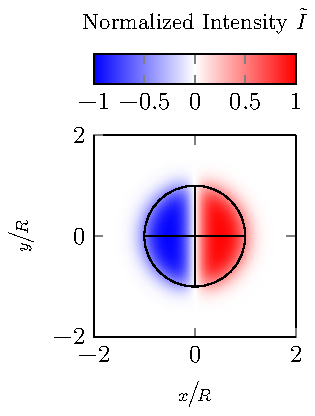
\includegraphics[]{Plots/cache/QPDx.pdf}
    \caption{Caption}
    \label{fig:Th-QPDx}
  \end{subfigure}
  \hfill
  \begin{subfigure}[b]{0.3\textwidth}
    \centering
    % \tikzsetnextfilename{QPDy}

\renewcommand{\tikzHelper}{
  \draw[black] (-1,0,0)--(1,0,0);
  \draw[black] (0,-1,0)--(0,1,0);
  \draw[black] (0,0,0) circle (1);

  \draw[black, dotted] (-1.5,0,0) -- (1.5,0,0);
  \draw[black, dotted] (-1.5,-0.6,0) -- (1.5,-0.6,0);
  \draw[black, dotted] (-1.5,0.6,0) -- (1.5,0.6,0);
}

\pgfplotsset{%
    colormap={bwr}{
      color=(blue);
      color=(white);
      color=(red);
    }%
}

\begin{tikzpicture}
  \begin{axis}[view={0}{90},
      xlabel=$\sfrac{x_{0}}{\RA}$,
      yticklabels={,,},
      point meta min=-1,
      point meta max=1,
      height=48mm,
      width=48mm,
      colorbar,
      colorbar horizontal,
      colorbar style={
        title={\footnotesize Normalized Intensity $\normalized{\intensity}$},
        at={(0,1.4)},
        anchor=north west,
        xtick={-1,0,1},
      }
    ]
      \addplot3[surf,mesh/rows=99,shader=interp] table[x=x,y=y,z=Vx] 
      {\relPath/10_Figures/TikZ/V_mat.dat};
    \tikzHelper
  \end{axis}
\end{tikzpicture}

    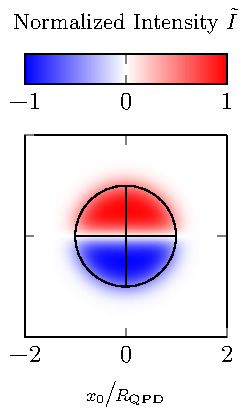
\includegraphics[]{Plots/cache/QPDy.pdf}
    \caption{Caption}
    \label{fig:Th-QPDy}
  \end{subfigure}
  \hfill
  \begin{subfigure}[b]{0.3\textwidth}
    \centering
    % \tikzsetnextfilename{QPDt}

\begin{tikzpicture}
  \begin{axis}[view={0}{90},
      xlabel=$\sfrac{x_{0}}{\RA}$,
      yticklabels={,,},
      height=48mm,
      width=48mm,
      colormap name=WhiteOr,
      colorbar,
      colorbar horizontal,
      colorbar style={
        title={\footnotesize Normalized Voltage $\normalized{V}_{t}$},
        at={(0,1.4)},
        anchor=north west,
        xtick={0,0.5,1},
      }
    ]
      \addplot3[surf,mesh/rows=99,shader=interp] table[x=x,y=y,z=V] 
      {\relPath/10_Figures/TikZ/V_mat.dat};

  \draw[black] (-1,0,0)--(1,0,0);
  \draw[black] (0,-1,0)--(0,1,0);
  \draw[black] (0,0,0) circle (1);

  \draw[black, dotted] (-1.5,0,0) -- (1.5,0,0);
  \draw[black, dotted] (-1.5,-0.6,0) -- (1.5,-0.6,0);
  \draw[black, dotted] (-1.5,0.6,0) -- (1.5,0.6,0);
  \end{axis}
\end{tikzpicture}

    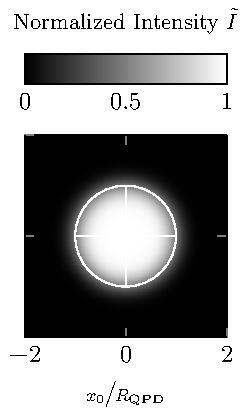
\includegraphics[]{Plots/cache/QPDt.pdf}
    \caption{Caption}
    \label{fig:Th-QPDt}
  \end{subfigure}
  \caption{QPDs}
  \label{fig:QPDs}
\end{figure}

\lipsum[1-2]

non-magnetic approximation

Fresnel equations specify the relation of the incident, reflected, and 
transmitted electrical field of an electromagnetic wave



power of electromagnetic wave

\cite[Chapter 7]{Jackson2013}


for plane emw in free space with $\mu_{\MR{r}} = 1$ (non-magnetic)

\begin{equation}
  \intensity = \timeaverage{\abs{\vb{S}}} = 
  \timeaverage{\abs{\vb{E}_{0}\times\vb{H}_{0}}} = 
  \frac{1}{2}\,\frac{\refraction}{Z_{0}}\,\abs{\vb{E}_{0}}^{2} = 
  \frac{1}{2}\,\refraction\,c\epsilon_{0}\,\abs{\vb{E}_{0}}^{2}
\end{equation}

\begin{equation}
  P = \intensity\,A \propto \refraction\,\abs{\vb{E}_{0}}^{2}\,A
\end{equation}

\begin{equation}
  P_{\MR{i}} = P_{\MR{r}} + P_{\MR{t}}
\end{equation}


\begin{equation}
  \fresnelR_{i} = \frac{P_{\MR{r}}}{P_{\MR{i}}} = 
  \frac{\intensity_{\MR{r}}\,\nf\,w_{\MR{r}}}{\intensity_{\MR{i}}\,\nf\,w_{\MR{i}}} 
  =\frac{\abs{\fresnelr_{i}\,\vb{E}_{0}}^{2}}{\abs{\vb{E}_{0}}^{2}} = 
  \fresnelr_{i}^{2}
\end{equation}

\begin{equation}
  \fresnelT_{i} = \frac{P_{\MR{t}}}{P_{\MR{i}}} = 
  \frac{\intensity_{\MR{t}}\,\ns\,w_{\MR{t}}}{\intensity_{\MR{i}}\,\nf\,w_{\MR{i}}} 
  =\frac{\abs{\fresnelt_{i}\,\vb{E}_{0}}^{2}}{\abs{\vb{E}_{0}}^{2}}\,\frac{\ns\,w_{\MR{t}}}{\nf\,w_{\MR{i}}} 
  = \fresnelt_{i}^{2}\,\frac{\ns\,\cos\transmitted}{\nf\,\cos\incident}
\end{equation}


% \begin{subequations}
% \begin{align}
  % \fresnelR_{\MR{s,p}} & = \resnelr_{\MR{s,p}}^{2} 
  % \label{eq:Th-fresnel-R}\\
  % \fresnelT_{\MR{s,p}} & = \fresnelt_{\MR{s,p}}^{2}\,
  % \frac{\ns\,\cos\reflected}{\nf\,\cos\incident}
  % \label{eq:Th-fresnel-T}
% \end{align}
% \end{subequations}

\begin{equation}
  \fresnelR + \fresnelT = 
  \frac{\fresnelR_{\MR{s}}+\fresnelR_{\MR{p}}}{2} +
  \frac{\fresnelT_{\MR{s}}+\fresnelT_{\MR{p}}}{2} = 1 
  \label{eq:Th-fresnel}
\end{equation}

\begin{subequations}
  \begin{alignat}{2}
  P_{\MR{t}}^{(1)} & = \fresnelT\,P_{\MR{i}}^{(1)} & \\
  P_{\MR{r}}^{(2)} & = \fresnelR\,P_{\MR{t}}^{(1)} & = 
  \fresnelR\fresnelT\,P_{\MR{i}}^{(1)} \\
  P_{\MR{t}}^{(2)} & = \fresnelT\,P_{\MR{t}}^{(1)} & = 
  \fresnelT^{2}\,P_{\MR{i}}^{(1)} > 0.99\,P_{\MR{i}}^{(1)}
\end{alignat}
\end{subequations}



\begin{figure}[htp]
  \centering
  % \tikzsetnextfilename{voltages_over_x}
%%%%%%%
% READ TABLE
%%%%%%%
\pgfplotstableread{\relPath/10_Figures/TikZ/V_line.dat}{\data}

\renewcommand{\tikzHelper}{
    \filldraw[black!10!, opacity=0.5] (-1,-1.1) rectangle (1,1.1);
    \filldraw[black!30!, opacity=0.5] (-0.15,-1.1) rectangle (0.15,1.1);
}

\begin{tikzpicture}
\begin{groupplot}[
    group style={
        group name=myplot,
        group size= 1 by 3,
        vertical sep=8mm,
        },
    height=40mm,
    width=120mm,
    ymin=-1.1,
    ymax=1.1,
    % legend style={fill=black,draw=white,},
    ]
    \nextgroupplot[
    % ylabel={$\tilde{I}$},
      xticklabels={,,},
      title={$y_{0} = \sfrac{0.6}{\RA}$},
      title style={yshift=-2mm},
      ]
      \tikzHelper
      \addplot[] table[x=x,y=Vy_3] {\data};
      \addlegendentry{$V_{\MR{x}}$};
      \addplot[dotted] table[x=x,y=Vx_3] {\data};
      \addlegendentry{$V_{\MR{y}}$};
      \addplot[dashed] table[x=x,y=V_3] {\data};
      \addlegendentry{$V_{\MR{t}}$};

      \draw[ultra thick, red, dashdotted] (axis cs:-0.4,-1.4026) -- (axis 
      cs:0.4,1.4026);

    \nextgroupplot[
      % ylabel={$\tilde{I}$},
      title={$y_{0} = \sfrac{0}{\RA}$},
      title style={yshift=-2mm},
      xticklabels={,,},
      ylabel={Normalized Intensity $\normalized{\intensity}$},
      every axis y label/.append style={at=(ticklabel cs:0.5)}
      ]
      \tikzHelper
      \addplot[] table[x=x,y=Vy_2] {\data};
      \addplot[dotted] table[x=x,y=Vx_2] {\data};
      \addplot[dashed] table[x=x,y=V_2] {\data};

      \draw[ultra thick, red, dashdotted] (axis cs:-0.4,-1.4795) -- (axis 
      cs:0.4,1.4795);
    \nextgroupplot[
      % ylabel={$\tilde{I}$},
      xlabel={$\sfrac{x_{0}}{\RA}$},
      title={$y_{0} = \sfrac{-0.6}{\RA}$},
      title style={yshift=-2mm},
      ]
      \tikzHelper
      \addplot[] table[x=x,y=Vy_1] {\data};
      \addplot[dotted] table[x=x,y=Vx_1] {\data};
      \addplot[dashed] table[x=x,y=V_1] {\data};

      \draw[ultra thick, red, dashdotted] (axis cs:-0.4,-1.4026) -- (axis 
      cs:0.4,1.4026);
\end{groupplot}
\end{tikzpicture}

  \includegraphics[]{Plots/cache/voltages_over_x.pdf}
  \caption{Fresnel}
  \label{fig:Th-voltages_over_x}
\end{figure}
